%----------------------------------------------------------------------------------------
%	Inställningar och dokumentkonfiguration
%----------------------------------------------------------------------------------------

\documentclass[paper=a4, fontsize=11pt]{report} % A4-sida och 11 punkters fontstorlek

\usepackage[T1]{fontenc} % 8-bitarskodning som har 256 glyfer
\usepackage[english]{babel} % Svenskt språk(ändrat till engelska)
\usepackage[utf8]{inputenc} % För svenska tecken
\usepackage{dtklogos} % Logos
\usepackage{wallpaper} % Bakgrundsbild
\usepackage{fancyhdr} % Specialsidhuvud och sidfot
\usepackage{enumerate} 
\usepackage{hyperref}
\usepackage{textcomp}
\usepackage{xifthen}% provides \isempty test
\pagestyle{fancyplain} % Använd sidhuvud och sidfot på alla sidor
\fancyhead[L]{Laboration 2 -- 1DV020 -- VT15 -- Server administraion I} % Titel till vänster i sidhuvud
\fancyhead[C]{} % Tomt i mitten
\fancyhead[R]{} % Tomt till höger
\fancyfoot[L]{{\color{gray}\textcopyright \ 2015 Jacob Lindehoff, Kristoffer Schill}} % Tomt till vänster
\fancyfoot[C]{}  % Tomt i mitten
\fancyfoot[R]{\thepage} % Sidnumrering till höger i sidfoten
\renewcommand\thesection{\arabic{section}} % Section beter sig som i dokumentklassen article

\newcommand{\win}[1]{Microsoft Windows Server\ifthenelse{\isempty{#1}}{}{ #1}}
\newcommand{\gui}[0]{``Server with a GUI''}
\newcommand{\core}[0]{Windows Server Core}
%----------------------------------------------------------------------------------------
%	TITLE SECTION
%----------------------------------------------------------------------------------------
\newcommand\BackgroundPic{
    \put(-50,-50){
    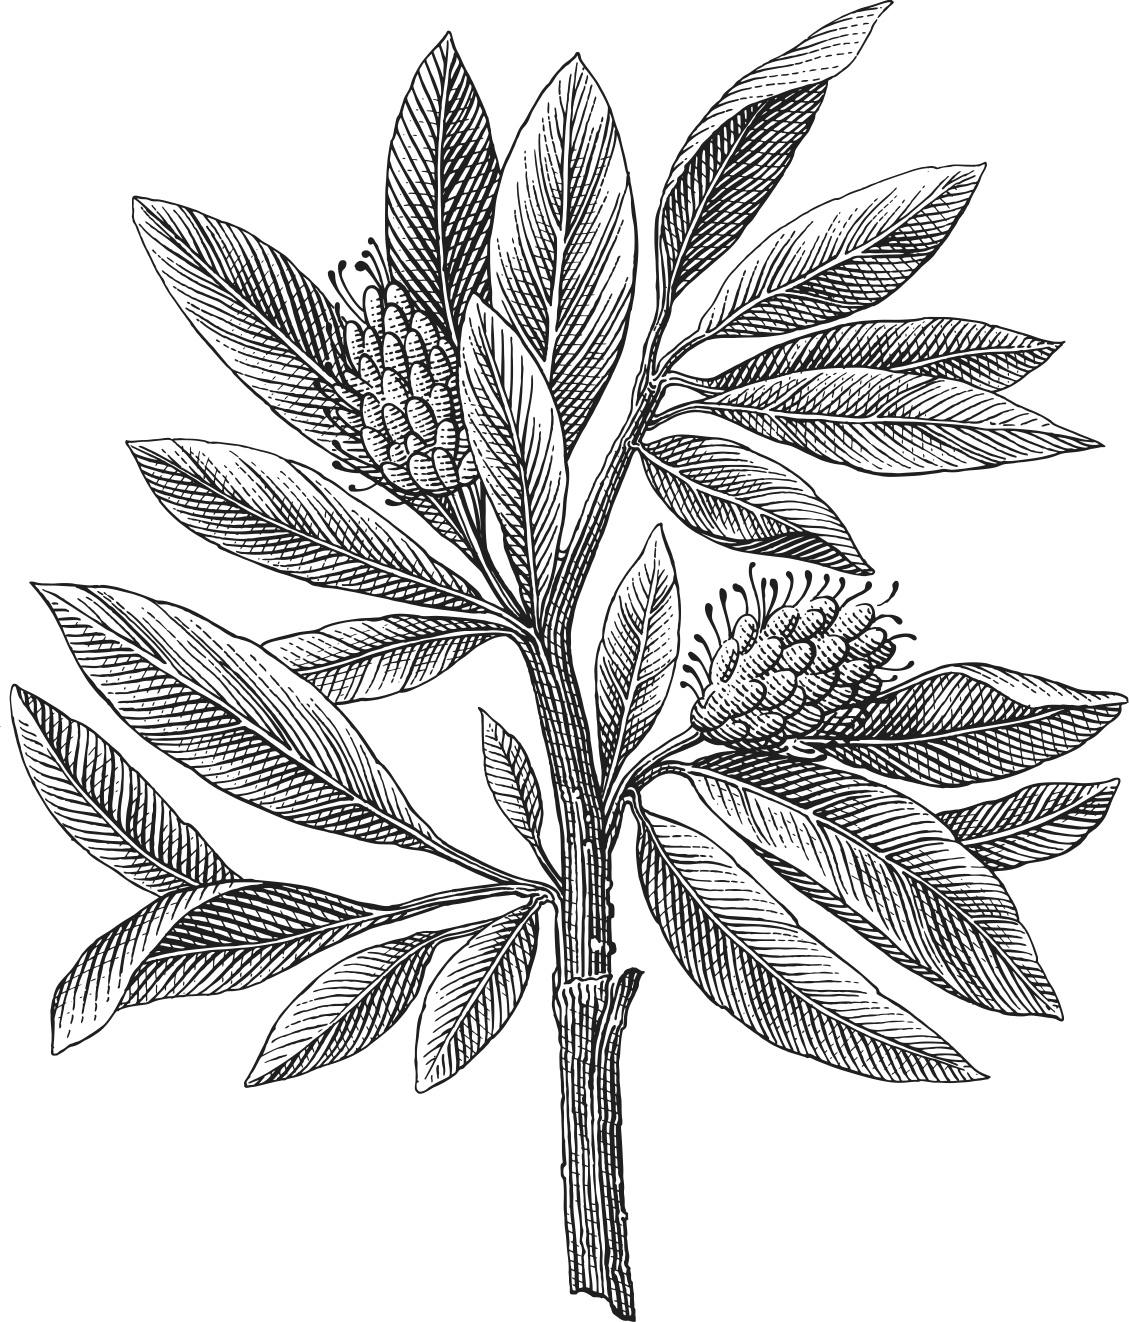
\includegraphics[keepaspectratio,scale=0.65]{lnu_etch.png} % Bakgrundsbild
    }
}
\newcommand\BackgroundPicLogo{
    \put(15,700){
    
\includegraphics[keepaspectratio,scale=0.10]{logo.png} % Logga i vänstra hörnet
    }
}

\newcommand{\horrule}[1]{\rule{\linewidth}{#1}} % Skapa hortisontell linje

\title{	\vspace{-10cm}
    \normalfont \normalsize
    \textsc{Linnéuniversitetet} \\ [25pt] % Universitetes namn
    \horrule{0.5pt} \\[0.4cm] % Tunn linje högst upp
    \huge Laboration 2\\ % Arbetes titel
	\large \textcolor{gray}{1DV020 -- Serveradministraion}
    \horrule{0.5pt} \\[0.4cm] % Tunn linje längst ner
}

% \author{Jacob Lindehoff} % Författarnas namn

\date{\normalsize\today} % Dagens datum

\begin{document}
\AddToShipoutPicture*{\BackgroundPic} % Lägger in backgrundsbild på första sidan
\AddToShipoutPicture*{\BackgroundPicLogo}
\maketitle % Skriv ut titeln
\noindent % Tabba inte in på första meningen

%------------------------------------------------
%	Introduction
%------------------------------------------------
\section{Introduction}

For this lab we will look into filesystems, partitioning, permissions and how these can be applied in a server enviroment. We will use the enviroment from the point we left of.

%------------------------------------------------
%	Deadline
%------------------------------------------------
\section{Deadline}

There are two laboratory sessions connected to this module, at these sessions you are given the opportunity to get help if so needed. To be able to finish the modules you are likely needed to spend more time on your own.

\paragraph{Accounting} You will show your work and demonstrate your progress at any of these lab session, prepare a small document with an overview of your configuration/setup if needed for overview.

\pagebreak
%------------------------------------------------
%	Uppgift
%------------------------------------------------
\section{Assignment}

Your task now is to do a few different operations on both the linux and the windows servers. First you will set up a fileserver that will serve out files from two different volumes each with different RAID setup. On the linux server we will use the terminal to partition a new hard drive to NTFS and mount it on the filesystem.

To do these tasks we need to add additional virtual harddrives to the servers. The procedure is simple: settings -> add -> hdd. As we are working with virtual harddrives they run on the physical harddrive and we will ofcourse not be able to see any increased performance. 

Limit the size of the hard drives to about 1 GB.
Windows Server:

Here you will create two volumes:

\begin{itemize}
	\item quick: Is intended to be fast and serve alot of data it is used but the data is not considered critical and fast access is more important. This one we will construct as an individiual drive letter.
	\item important: Here the data is crucial and here we have to implement another RAID soluition.  We also put it into an empty NTFS folder on the system.
\end{itemize}

Then we need to set up both of these as shares on the network and we will enforce some sharing rules - and for this task we will not add the users to the Active Directory but instead to the local system.

\begin{itemize}
	\item Create 3 users: Pelle, Lisa and Stina.
	\item Pelle and Lisa may read and write quick, Stina is only allowed to read it.
	\item Stina may read and write important, Lisa may read important.
\end{itemize}

Linux Server:

You will partition the new volume you just added into a functional NTFS drive using the terminal and fdisk. You shall then configure fstab so that on each reboot the drive is remounted.

Lisa, Pelle and Stina with a homefolder each (If you havn’t played around in /etc/adduser.conf you could use the command adduser and the /home/ folders will be located in /home/Pelle ...)

Make Samba share each homefolder so that the respective user can access his/her shares from here. Files created by any of the user should be owned by that user.

The users should only be allowed to read and access their respective folder.

\section{Requirements}
\label{tasks}

Aside from keeping the configuration where we left of(static ip's, firewalls , VMNet) It should be set up as in the Assignment. Firewall rules will be checked to be ‘decent’. Remember that if (as it should be) your firewall is properly setup you will need to make exception for the protocols you are implementing f.e. SMB and if you are using SWAT for samba you need to allow that traffic in.

As previously your configuration should survive a reboot.
    \begin{itemize}
        \item \textbf{Linux Server}
        \begin{itemize}
		\item one extra hdd partition as a functional NTFS, mounted on boot.
		\item 3 Users Stina, Pelle and Lisa.
		\item Each home directory is shared and can only be accessed by themself.
	\end{itemize}

	\item \textbf{Windows Server}
	\begin{itemize}
		\item Create the three local user accounts: Pelle, Lisa and Stina.
		\item Create one RAID solution from a few of your HDDs for quick file access.(Assume the virtual disks as physical disks) - quick
		\item Create one RAID solution from a few of your HDDs for secure file storage.(Assume the virtual disks as physical disks) - important
		\item quick should be mounted as seperate volume index.(f.e. E:)
		\item important should be mounted as a folder in your NTFS directory. (f.e. C: -> important)
		\item enforce ACL for "quick" so Pelle and Lisa may both read and write and Stina is only allowed to read.
		\item enforce ACL for "important" so Stina may read and write, Lisa may read and Pelle is not allowed to even read it.
	\end{itemize

\end{itemize}

\section{Workenviroment}
\label{enviroment}

	As previously we will be using VMware to accomplish this. For this assignment we only need to use the hosts on VMNet2 and the ISP Gateway for internet access.

\end{document}
